\chapter{Funciones de Legendre, Asociadas de Legendre y Arm\'onicos Esf\'ericos}

\section{E.D.O. Asociada de Legendre}
Substituyendo $x:=\cos\theta$ tendremos que la ecuaci'on diferencial \eqref{ecThHelm} para $\Theta(\theta)$ se transforma en 
\begin{eqnarray}
\frac{d}{dx}\left((1-x^2)\frac{dy}{dx}\right) +
\left[Q-\frac{m^2}{1-x^2}\right]\cdot y(x) = 0, \qquad x\in [-1,1],\label{est22}
\end{eqnarray}
de modo que, dada una soluci'on $y(x)$, la soluci'on de \eqref{ecThHelm} es dada por $\Theta(\theta)=y(\cos\theta)$. 

\subsection{E.D.O de Legendre}
En el caso $m=0$, la ecuaci'on (\ref{est22}) es llamada \textbf{ecuaci'on
diferencial de Legendre}:
\begin{equation}\label{ecLeg}
\frac{d}{dx}\left[\left(1-x^2 \right)\frac{dy}{dx}\right]+Qy=0, \qquad x\in [-1,1].
\end{equation}

 En la secci'on \ref{sec:FrobLeg} estudiaremos la soluci'on general de esta ecuaci'on, para valores arbitrarios de la constante $Q$. Ah'i verificaremos que 
\begin{quotation}
\textbf{Teorema:} La ecuaci'on \eqref{ecLeg} s'olo posee soluciones \textit{finitas en los puntos extremos} ($x=\pm 1$) si y s'olo si
\begin{equation}
Q=n(n+1),\qquad n=0, 1,2, \cdots,
\end{equation} 
es decir, s'olo si $Q=0,2,6,12,20,30,\dots$. En este caso las soluciones finitas son los \textbf{Polinomios de Legendre} de orden $n$. 
\end{quotation}

\subsection{Polinomios de Legendre y funci\'on generadora}
Antes de abordar el problema m'as general, introduciremos los polinomios de Legendre por medio de su \textbf{funci'on generadora}. Para esto, consideramos el siguiente argumento:

La funci'on (en coordenadas esf'ericas $(r,\theta,\varphi)$)
\begin{equation}\label{PsisolLap}
\Psi(r,\theta)=\frac{1}{\sqrt{r^2+a^2-2ar\cos\theta}}
\end{equation}
es una soluci'on axialmente sim'etrica (e.d. independiente de $\varphi$) de la ecuaci'on de Laplace. Esto puede verificarse f'acilmente a partir del potencial electrost'atico que genera una carga puntual de magnitud $q$ ubicada sobre el eje $z$, a una distancia $a$ del origen, que es determinado por la ley de Coulomb. Este potencial es precisamente $\phi=(q/4\pi\varepsilon_0)\Psi(r,\theta)$.

Expandiendo \eqref{PsisolLap} en potencias de $t:=a/r$, para $r>a$, obtenemos
\begin{align}
\Psi(r,\theta) &= \frac{1}{\sqrt{r^2+a^2-2ar\cos\theta}} \\
&= \frac{1}{r}\frac{1}{\sqrt{1+t^2-2xt}} \\
&= \frac{1}{r}\sum_{n=0}^\infty P_n(x)t^n \\
&= \frac{1}{a}\sum_{n=0}^\infty P_n(x)t^{n+1}, \label{solPntn+1}
\end{align}
donde hemos introducido nuevamente $x:=\cos\theta$. De esta forma, tenemos una soluci'on finita para todo $t<1$ que consiste en una superposici'on de soluciones separables $P_n(x)$ y $t^{n+1}$. Comparando esta soluci'on con \eqref{loes2} vemos que \eqref{solPntn+1} corresponde al caso particular en que $Q=n(n+1)$. Por lo tanto, esperamos que las funciones $P_n(x)$ satisfagan la ecuaci'on \eqref{ecLeg} en este caso.  

Con esta motivaci'on, podemos definir las funciones de Legendre de orden $n$, $P_n(x)$, como los \textit{coeficientes de la expansi'on en serie de Taylor de la ``funci'on generadora''}  $g(t,x):=(1-2xt+t^2)^{-1/2}$, tal que
\begin{equation}
g(t,x):=\frac{1}{\sqrt{1-2xt+t^2}}=\sum_{n=0}^{\infty}P_{n}(x)t^{n}.
\end{equation}
Equivalentemente, tenemos entonces que
\begin{equation}
P_n(x)=\frac{1}{n!}\left.\left[\frac{\partial^ng(t,x)}{\partial t^n}\right]\right|_{t=0}.
\end{equation}

\subsubsection{Expresiones expl'icitas}
Los primeros cuatro polinomios son
 \begin{align*}
  P_0(x) &= 1, &P_1(x) &= x,\\
  P_2(x) &= \frac 12(3x^2-1), &P_3(x) &= \frac 12(5x^3-3x),\\
  P_4(x) &= \frac{35 x^{4}}{8} - \frac{15 x^{2}}{4} + \frac{3}{8}, \qquad 
  &P_5(x) &= \frac{63 x^{5}}{8} - \frac{35 x^{3}}{4} + \frac{15 x}{8}.
 \end{align*}
 
\subsubsection{Serie de potencias}
Podemos encontrar una primera expresi'on para las funciones $P_n(x)$ en t'erminos de una serie de potencias. Para esto, podemos expandir la funci'on generadora en una serie, usando
\begin{equation}
(1-x)^{-1/2}=\sum_{n=0}^\infty\frac{(2n)!}{2^{2n}(n!)^2}x^n,
\end{equation}
con la identificaci'on $x\rightarrow 2xt-t^2$, de modo que
\begin{align}
g(t,x) &= \sum_{n=0}^\infty\frac{(2n)!}{2^{2n}(n!)^2}(2xt-t^2)^n \\
&= \sum_{n=0}^\infty\frac{(2n)!}{2^{2n}(n!)^2}t^n(2x-t)^n \\.
\end{align}
Empleamos ahora la expansi'on binomial,
\begin{equation}
(a+b)^n=\sum_{k=0}^n\frac{n!}{k!(n-k)!}a^{n-k}b^k,
\end{equation}
con $a=2x$ y $b=-t$. Entonces, podemos escribir
\begin{align}
g(t,x) 
&= \sum_{n=0}^\infty\frac{(2n)!}{2^{2n}(n!)^2}t^n \sum_{k=0}^n\frac{n!}{k!(n-k)!}(2x)^{n-k}(-t)^k\\
&= \sum_{n=0}^\infty\sum_{k=0}^n\frac{(-1)^k(2n)!}{2^{n+k}n!k!(n-k)!}x^{n-k}t^{n+k}.
\end{align}
Podemos expresar esta suma doble cambiando de variable de suma desde $(n,k)$ hasta $(\bar{n},k)$, con $\bar{n}:=n+k$. Esto implica reemplazar $n$ en la expresi'on anterior por $\bar{n}-k$ y el rango de variaci'on de estas variables. Si $\bar{n}=0,1,2,\dots$, entonces $k=0,1,\cdots,[\bar{n}/2]$, ya que en la suma original $n-k=\bar{n}-2k>0$. Por lo tanto
\begin{equation}
g(t,x)= \sum_{\bar{n}=0}^\infty\sum_{k=0}^{[\bar{n}/2]}\frac{(-1)^k(2\bar{n}-2k)!}{2^{\bar{n}}k!(\bar{n}-k)!(\bar{n}-2k)!} x^{\bar{n}-2k}t^{\bar{n}},
\end{equation}
y por lo tanto
\begin{equation}\label{seriePn}
P_n(x)= \sum_{k=0}^{[n/2]}\frac{(-1)^{k}(2n-2k)!}{2^nk!(n-k)!(n-2k)!}x^{n-2k}.
\end{equation}

\subsubsection{Propiedades}
Los polinomios de Legendre satisfacen las siguientes propiedades:
\begin{itemize}
\item Normalizaci'on
\begin{equation}
     P_n(1) = 1.
\end{equation}
En otras palabras, los $P_n$ son normalizados de modo que para $x=1$ ellos
asumen siempre el valor $1$.
 \item Simetr'ia
\begin{equation}
P_n(-x) = (-1)^n P_n(x).
\end{equation}
Los polinomios $P_n$ son funciones sim'etricas si $n$ es par y antisim'etricas
si $n$ es impar

\item Valor en el origen:
\begin{equation}\label{Pn0}
P_n(0)=\left\{\begin{array}{cl}
0 & \text{si } n \text{ par} \\
\frac{(-1)^m(2m)!}{2^{2m}(m!)^2} & \text{si } n=2m \text{ (par)}
\end{array}\right. .
\end{equation}

\item Completitud: Los polinomios de Legendre $P_n$ forman un conjunto
completo de funciones definidas en $[-1,1]$.
 \end{itemize}

\begin{figure}[H]
\centering
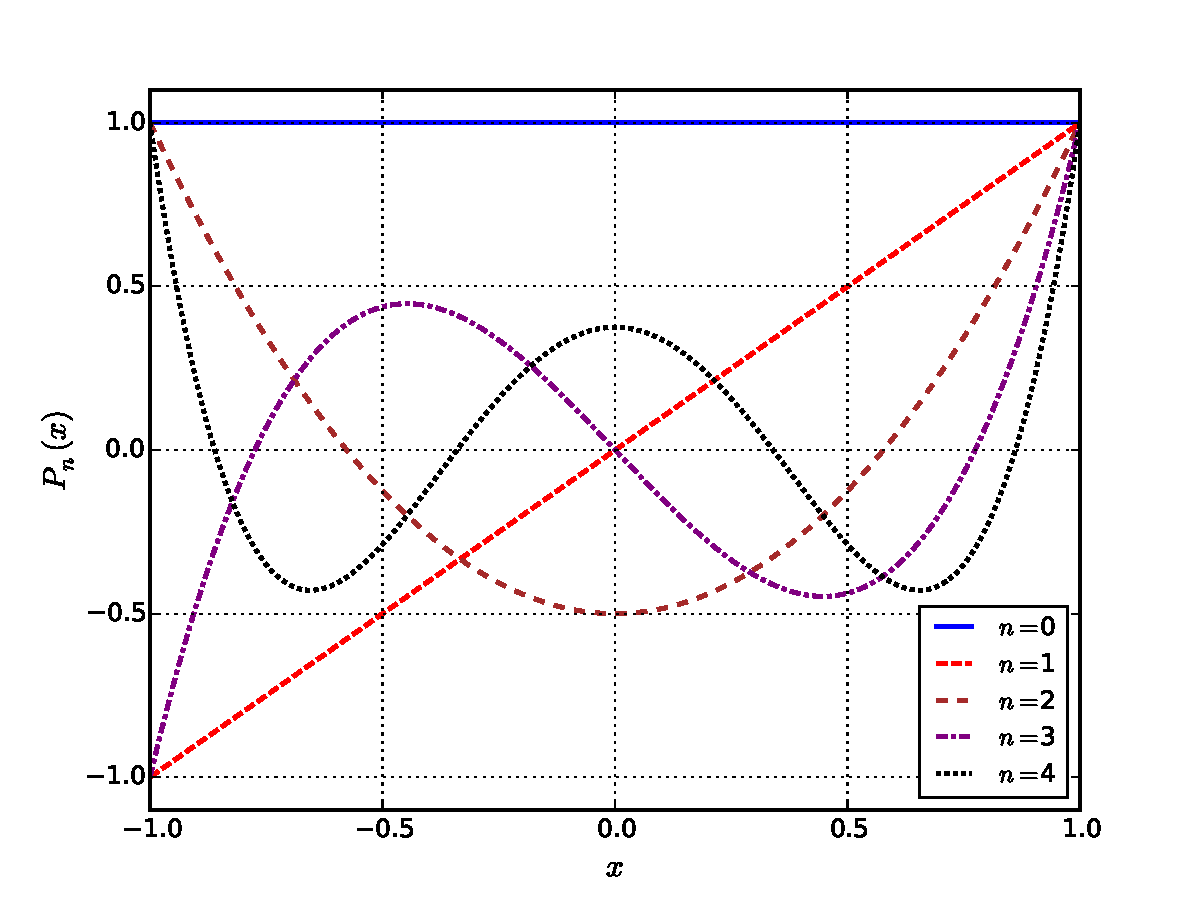
\includegraphics[angle=0,width=0.8\textwidth]{figs/fig-Legendre-P.pdf}
\caption{Primeros cinco polinomios de Legendre. C'odigo Python disponible \href{https://github.com/gfrubi/FM2/blob/master/figuras-editables/fig-Legendre.py}{aqu\'i}.}
\label{fig-Pn}
\end{figure}

\begin{figure}[H]
\centering
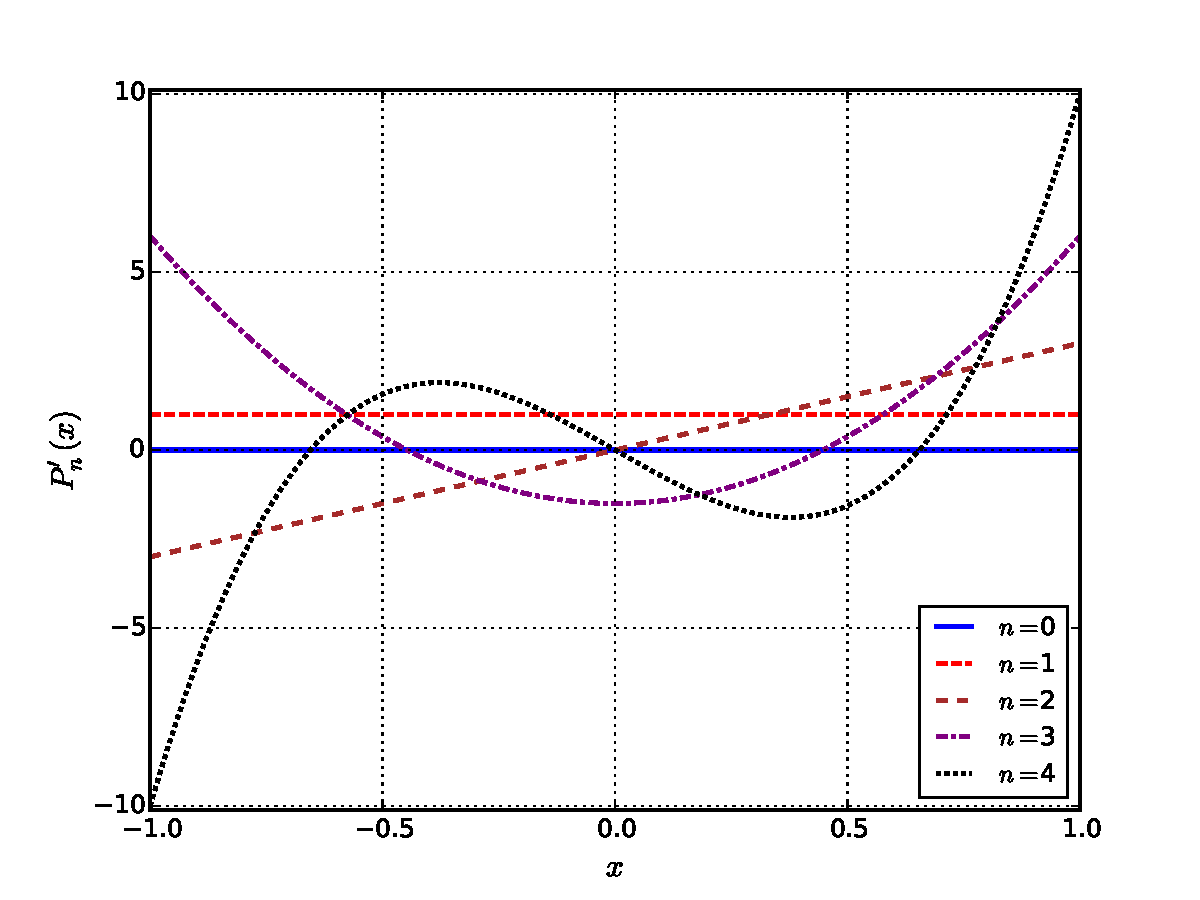
\includegraphics[angle=0,width=0.8\textwidth]{figs/fig-Legendre-der-P.pdf}
\caption{Derivada de los primeros cinco polinomios de Legendre. C'odigo Python disponible \href{https://github.com/gfrubi/FM2/blob/master/figuras-editables/fig-Legendre.py}{aqu\'i}.}
\label{fig-Pnp}
\end{figure}



\subsubsection{F'ormula de Rodrigues}

\begin{equation}
P_{n}(x)=\frac{1}{2^{n}n!}\frac{d^{n}}{dx^{n}}(x^2-1)^{n}
\end{equation}


\subsubsection{Relaciones de recurrencia}
\begin{gather}
nP_{n-1}(x)+(n+1)P_{n+1}(x)=(2n+1)\,x\,P_n(x), \\
(2n+1)P_n(x)=P'_{n+1}(x)-P'_{n-1}(x).
\end{gather}

\subsection{Relaci'on de ortogonalidad}
\begin{equation}
\frac{d\ }{dx}\left[(1 - x^2) P_n' \right]+ n (n + 1) P_n=0, \quad
\frac{d\ }{dx}\left[(1 - x^2) P_m' \right]+ m (m + 1) P_m=0 .
\end{equation}

\begin{gather}
[n (n + 1) - m (m + 1)]\int_{-1}^1 P_n(x) P_m(x)\,d x = 0 
\\
\int_{-1}^1 P_n(x) P_m(x)\,d x = 0, \qquad n\neq m.
\end{gather}
\begin{equation}\label{ortoPn}
\boxed{\int_{-1}^{1}P_n(x)P_m(x)\,dx=\frac{2}{2n+1}\delta_{mn}.}
\end{equation}
Como los polinomios de Legendre son ortogonales, se sigue que son \textit{linealmente independientes} (l.i.), ya que
\begin{equation}
\sum_{n=0}^\infty a_nP_n(x)=0,
\end{equation}
s'i y s'olo si $a_n=0$.
\subsection{Series de Legendre}
Es posible expandir una funci'on $f(x)$, definida en el intervalo $x\in[-1,1]$ y continua por tramos, en una \textbf{serie de Legendre}, es decir, en una suma de polinomios de Legendre, de la forma
\begin{equation}
f(x)=\sum_{n=0}^\infty a_nP_n(x),
\end{equation}
en el sentido que la serie coverge en media a la funci'on $f(x)$ para todo $x$ en $[-1,1]$.

Podemos encontrar una expresi'on para los coeficientes usando la relaci'on de ortogonalidad \eqref{ortoPn}:
\begin{equation}
a_n=\frac{2n+1}{2}\int_{-1}^1 f(x)P_n(x)\,dx.
\end{equation}
\subsubsection{Expansi'on de Legendre de la Delta de Dirac}
En el caso en que $f(x)=\delta(x-a)$ tendremos que
\begin{align}
a_n &= \frac{2n+1}{2}\int_{-1}^1 \delta(x-a)P_n(x)\,dx \\
&= \frac{2n+1}{2}P_n(a),
\end{align}
y entonces
\begin{equation}
\delta(x-a)=\sum_{n=0}^\infty \frac{2n+1}{2}P_n(a)P_n(x).
\end{equation}
En particular, usando \eqref{Pn0} encontramos
\begin{equation}
\delta(x)=\sum_{m=0}^\infty \frac{(-1)^m(4m+1)(2m)!}{2^{2m+1}(m!)^2}P_{2m}(x).
\end{equation}

\begin{figure}[H]
\centering
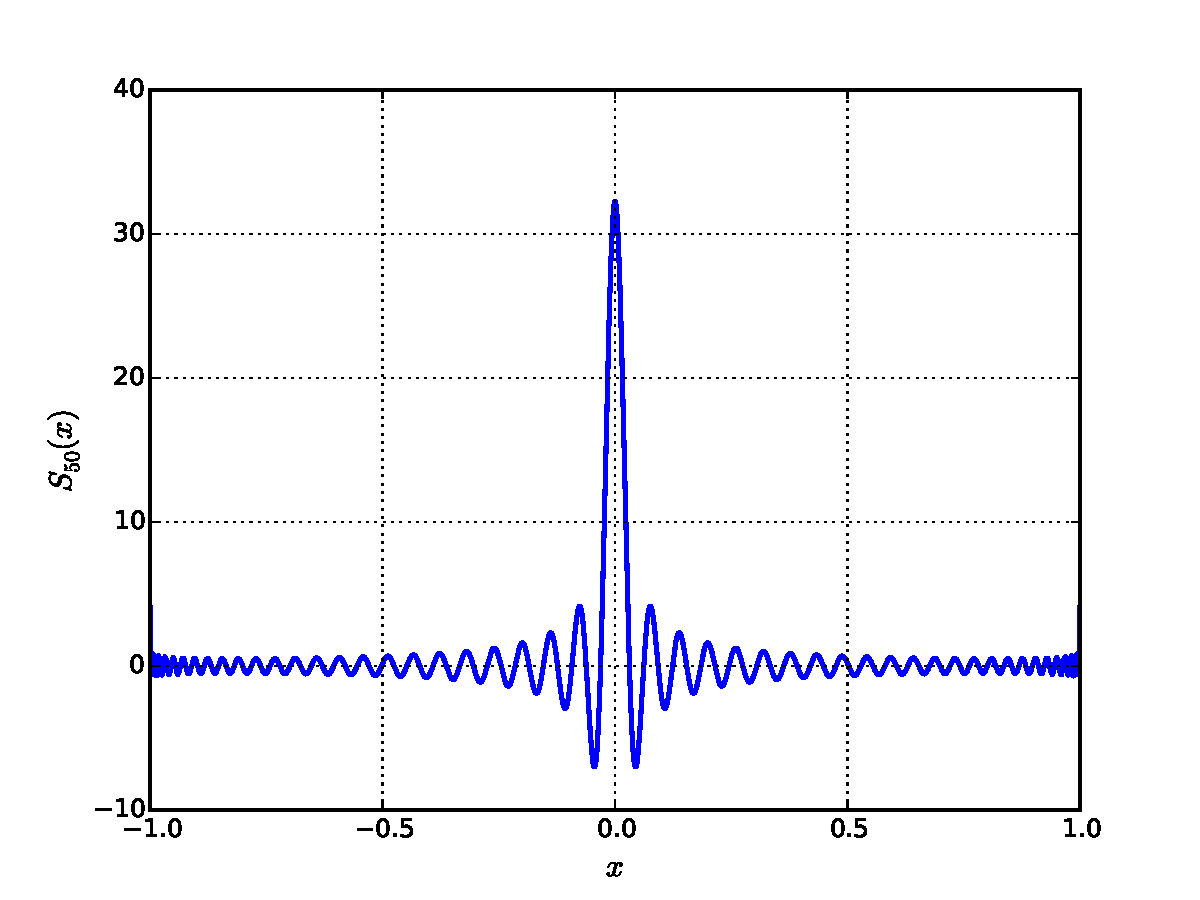
\includegraphics[angle=0,width=0.8\textwidth]{figs/fig-Legendre-serie-Delta.pdf}
\caption{Serie (truncada a orden $50$) de la serie de Legendre de $\delta(x)$.}
\label{fig-DSL}
\end{figure}

\subsection{Soluci'on en serie de Potencias (M'etodo de Frobenius)}\label{sec:FrobLeg}

Primero escribimos la E.D.O. de Legendre \eqref{ecLeg} en su forma estandar:
\begin{equation}
\label{eqn_legendre_eqn}
\left( 1 - x^2 \right) y'' - 2 x y' + Q y = 0,
\end{equation}
o bien
\begin{equation}
\label{eqn_legendre_eqn_norm}
y'' - \frac{2 x}{1 - x^2} y' + \frac{ Q }{1 - x^2} y = 0.
\end{equation}
Como los coeficientes de $y'$ y $y$ son funciones anal'iticas en la vencindad de 
$x = 0$, podemos encontrar una soluci'on en serie de Taylor en torno a ese punto:
\begin{align*}
y &= \sum_{k=0}^\infty a_k x^k ,
\\
y' &= \sum_{k=0}^\infty k a_k x^{k-1} ,
\\
y'' &= \sum_{k=2}^\infty (k-1) k a_k x^{k-2} 
\\
&= \sum_{k=0}^\infty (k+1) (k+2) a_{k+2} x^k.
\end{align*}
Sustituyendo estas series en \eqref{eqn_legendre_eqn} obtenemos
\begin{equation}
\sum_{k=0}^\infty (k+1) (k+2) a_{k+2} x^k
- \sum_{k=0}^\infty (k-1) k a_k x^k
- 2 \sum_{k=0}^\infty k a_k x^k
+ Q \sum_{k=0}^\infty a_k x^k= 0 ,
\end{equation}
\begin{equation}
\sum_{k=0}^\infty \left[ (k+1)(k+2) a_{k+2} - \left( (k-1) k + 2 k - Q \right) a_k \right] x^k = 0.
\end{equation}
Igualando los coeficientes de cada t'ermino $x^k$ obtenemos las relaciones de recurrencia
\begin{equation}\label{recLeg}
a_{k+2} = \frac{ k (k+1) - Q}{ (k+1)(k+2) } a_k, \qquad k=0,1,2,\cdots.
\end{equation}
A partir de ellas, podemos encontrar todos los coeficientes $a_k$, con $k\ge 2$ a partir de $a_0$ y $a_1$:
\begin{equation}
a_k =
\begin{cases}
\displaystyle{
\frac{a_0}{k!} \prod_{\substack{l=0 \\ l \text{ par}}}^{k-2} 
\left( l (l+1) - Q \right),
}
&k \text{ par}, 
\\
\displaystyle{
\frac{a_1}{k!} \prod_{\substack{l=1 \\ l \text{ impar}}}^{k-2} \left( l (l+1) - Q \right),
}
&k \text{ impar} .
\end{cases}
\end{equation}

Por lo tanto, la soluci'on general ser'a una combinaci'on lineal de la forma
\begin{equation}
y(x)=a_0y_1(x)+a_1y_2(x),
\end{equation}
donde $y_1(x)$ es una funci'on par en $x$ e $y_2(x)$ es una funci'on impar en $x$, dadas por
\begin{equation}
y_1(x) = \sum_{m= 0}^\infty \left(\frac{1}{(2m)!}
\prod_{\substack{l=0 \\ l \text{ par}}}^{2m-2}
\left( l (l+1) -Q \right) \right) x^{2m}=:\sum_{m= 0}^\infty b_m x^{2m}, \label{y1}
\end{equation}
\begin{equation}
y_2(x) = \sum_{m=0}^\infty\left( \frac{1}{(2m+1)!}
\prod_{\substack{l=1 \\ l \text{ impar}}}^{2m-1}
\left( l (l+1) - Q \right) \right) x^{2m+1}
=:\sum_{m= 0}^\infty c_m x^{2m+1}. \label{y2}
\end{equation}

En general, tanto $y_1(x)$ como $y_2(x)$ ser'an series infinitas, ya que los correspondientes coeficientes de cada $x^k$, dados por un producto de factores, ser'an no nulos \textit{excepto si existe un valor de $l$ tal que} $l(l+1)-Q=0$. Esto s'olo ocurrir'a si la constante $Q$ es de la forma $Q=n(n+1)$, con alg'un valor de $n=0,1,2,\cdots$. Si este es el caso, entonces una de las series se \textit{truncar'a}, reduci'endose a un polinomio.

\subsubsection{Convergencia}
Analicemos primero el caso gen'erico en que $Q\neq n(n+1)$. Como dijimos, las dos soluciones l.i. $y_1(x)$ e $y_2(x)$ ser'an series infinitas, debiendo por tanto analizar su convergencia.

Consideramos primero el \textbf{test de D'\,Alambert}\footnote{Tambi'en llamado ``Cauchy ratio test'': Si $\lim_{n\to\infty}\left|u_{n+1}/u_n\right|<1$ entonces $\sum_{n=0}^\infty u_n$ es una serie convergente. Si $\lim_{n\to\infty}\left|u_{n+1}/u_n\right|>1$ la serie es divergente. Si $\lim_{n\to\infty}\left|u_{n+1}/u_n\right|=1$ el test de Cauchy no suministra informaci'on. Ver, por ejemplo, \cite{Arfken}, secci'on 5.2.}. Para el caso de $y_1(x)$ tenemos que $y_1(x)=\sum_{m=0}^\infty u_m$, con 
\begin{equation}
u_m=\frac{x^{2m}}{(2m)!}
\prod_{\substack{l=0 \\ l \text{ par}}}^{2m-2}
\left( l (l+1) -Q \right)=a_{2m}x^{2m},
\end{equation}
y entonces
\begin{align}
\lim_{m\to\infty}\left|\frac{u_{m+1}}{u_m}\right| 
&=\lim_{m\to\infty}\left|\frac{b_{m+1}x^{2m+2}}{b_mx^{2m}}\right|
= \lim_{m\to\infty}\left|\frac{a_{2m+2}}{a_{2m}}\right| x^2 \\
&= \lim_{m\to\infty}\left|\frac{(2m(2m+1)-Q)}{(2m+1)(2m+2)}\right| x^2
= x^2.
\end{align}

Por lo tanto, podemos afirmar que $y_1(x)$ es convergente para $|x|<1$. Para analizar la convergencia cuando $x=\pm 1$ podemos usar el test de Gauss\footnote{Si $u_n>0$ $\forall n$ y $u_n/u_{n+1}=1+h/n+B(n)/n^2$ donde $h$ es una constante y $B(n)$ una funci'on acotada de $n$ para $n\to\infty$ entonces la serie $\sum_n u_n$ converge si $h>1$ y diverge si $h\le 1$. Ver, por ejemplo, \cite{Arfken}, secci'on 5.2.}. En nuestro caso ($u_m>0$ para $m$ suficientemente grande) y 
\begin{equation}
\frac{u_m}{u_{m+1}}=\frac{(2m+1)(2m+2)}{(2m(2m+1)-Q)}=\left[1+\frac{1}{m}+\frac{Q}{8m^2}\left(2+\frac{1}{m}+O(\frac{1}{m^2})\right)\right].
\end{equation}
Por lo tanto, $h=1$ y entonces $y_1(x)$ es una serie divergente en $x=\pm 1$.

An'alogamente, puede verificarse que las mismas conclusiones son v'alidas para $y_2(x)$. En resumen, 

\begin{quote}
si $Q\neq n(n+1)$ las soluciones de la ec. de Legendre son divergentes en los extremos del intervalo considerado, e.d. en $x=\pm 1$.
\end{quote}

\subsubsection{Caso $Q=n(n+1)$}
Analicemos ahora con m'as detalle el caso en que $Q=n(n+1)$, puesto que aqu'i obtendremos series truncadas (es decir, polinomios) que naturalmente son funciones finitas en todo el intervalo considerado, incluyendo los extremos. De (\ref{recLeg}) vemos que $a_{n+2}=0$, y por consiguiente todos los coeficientes de orden superior de la forma $a_{n+2p}$ ser'an nulos, con $p=1,2,\cdots$. Por lo tanto, si $n$ es par entonces ser'a la serie $y_1(x)$ la que se truncar'a, mientras que $y_2(x)$ continuar'a siendo una serie infinita. Por otro lado, si $n$ es impar $y_1(x)$ tendr'a infinitos t'erminos, mientras que $y_2(x)$ se reduce a un polinomio. El orden del correspondiente polinomio truncado es $n$ en ambos casos ($a_n$ es el 'ultimo t'ermino no nulo). Esperamos por lo tanto que estos polinomios sean proporcionales a los polinomios de Legendre de orden $n$. A partir de (\ref{y1}) e (\ref{y2}), y usando $l(l+1)-n(n+1)=(l-n)(l+n+1)$ encontramos que
\begin{equation}\label{y1n1}
y_{1,n}(x) = \sum_{m= 0}^{n/2}b_mx^{2m}, \qquad b_m=\frac{1}{(2m)!}
\prod_{\substack{l=0 \\ l \text{ par}}}^{2m-2}
(l-n)(l+n+1), \qquad n\text{ par},
\end{equation}
\begin{equation}\label{y2n1}
y_{2,n}(x)=\sum_{m= 0}^{(n-1)/2}c_mx^{2m+1}, \qquad c_m =\frac{1}{(2m+1)!}
\prod_{\substack{l=1 \\ l \text{ impar}}}^{2m-1}
 (l-n)(l+n+1), \qquad n\text{ impar}.
\end{equation}

Luego de algo de 'algebra, podemos verificar que
\begin{equation}
b_m=\frac{(-1)^m}{(2m)!}\frac{(n+2m)![(n/2)!]^2}{n!(n/2-m)!(n/2+m)!},
\end{equation}
y con ello, podemos escribir la soluci'on $y_{1,n}$ como
\begin{align}
y_{1,n}(x) &= \frac{[(n/2)!]^2}{n!}\sum_{m=0}^{n/2}\frac{(-1)^m}{(2m)!}\frac{(n+2m)!}{(n/2-m)!(n/2+m)!}x^{2m}.
\end{align}
Finalmente, cambiando 'indice de suma desde $m$ hasta $k:=n/2-m$, de modo que $2m=n-2k$, podemos escribir
\begin{align}
y_{1,n}(x) &= \frac{[(n/2)!]^2}{n!}\sum_{k=0}^{n/2}\frac{(-1)^{n/2-k}}{(n-2k)!}\frac{(2n-2k)!}{k!(n-k)!}x^{n-2k} \\
&= (-1)^{n/2}\frac{[(n/2)!]^2}{n!}\sum_{k=0}^{n/2}\frac{(-1)^{k}}{(n-2k)!}\frac{(2n-2k)!}{k!(n-k)!}x^{n-2k} \\
&= (-1)^{n/2}\frac{[(n/2)!]^2}{n!} 2^n P_n(x), \qquad n=0,2,4,\cdots. \label{y1Pn}
\end{align}
En el 'ultimo paso hemos identificado la serie de potencias \eqref{seriePn} de los polonomios de Legendre.

An'alogamente, para $n$ impar podemos expresar los coeficientes $c_m$ como
\begin{equation}
c_m=\frac{(-1)^m}{(2m+1)!}\frac{(n+2m)![\left(\frac{n-1}{2}\right)!]^2}{n!\left(\frac{n-2m-1}{2}\right)!\left(\frac{n+2m-1}{2}\right)!},
\end{equation}
de modo que
\begin{align}
y_{2,n}(x) &= \sum_{m=0}^{(n-1)/2}\frac{(-1)^m}{(2m+1)!}\frac{(n+2m)![\left(\frac{n-1}{2}\right)!]^2}{n!\left(\frac{n-2m-1}{2}\right)!\left(\frac{n+2m-1}{2}\right)!}x^{2m+1} \\
&= \frac{[\left(\frac{n-1}{2}\right)!]^2}{n!}\sum_{m=0}^{(n-1)/2}\frac{(-1)^m}{(2m+1)!}\frac{(n+2m)!}{\left(\frac{n-2m-1}{2}\right)!\left(\frac{n+2m-1}{2}\right)!}x^{2m+1}
\end{align}
Cambiamos ahora 'indice de suma, definiendo $k$ tal que $2m+1=n-2k$, y encontramos
\begin{align}
y_{2,n}(x) &= \frac{[n/2]!^2}{n!}\sum_{k=0}^{(n-1)/2}\frac{(-1)^{\frac{n-2k-1}{2}}}{(n-2k)!}\frac{(2n-2k-1)!}{k!(n-k-1)!}\,x^{n-2k} \\
&= \frac{[n/2]!^2}{n!}(-1)^{(n-1)/2}\sum_{k=0}^{[n/2]}\frac{(-1)^k}{(n-2k)!}\frac{(2n-2k)!}{(2n-2k)}\frac{1}{k!}\frac{(n-k)}{(n-k)!}\,x^{n-2k} \\
&= \frac{[n/2]!^2}{n!}\frac{(-1)^{[n/2]}}{2}\sum_{k=0}^{[n/2]}\frac{(-1)^k}{(n-2k)!}\frac{(2n-2k)!}{k!(n-k)!}\,x^{n-2k} \\
&= \frac{[n/2]!^2}{n!}(-1)^{[n/2]}2^{n-1} P_n(x), \qquad n=1,3,5,\cdots. \label{y2Pn}
\end{align}
En resumen, usando una notaci'on algo m'as compacta, podemos escribir:
\begin{equation}
P_n(x):=(-1)^{[n/2]}2^{-2[n/2]}\frac{n!}{[n/2]!^2} \times
	\begin{cases}
	y_{1,n}(x) , & n \text{ par}\\
	y_{2,n}(x), & n \text{ impar}.
	\end{cases}
\end{equation}

\subsection{Funciones de Legendre de segunda especie}
Como hemos visto, en el caso en que $Q=n(n+1)$ una de las series ($y_1$ si $n$ es par, $y_2$ si $n$ es impar) se trunca, reduci'endose (salvo factores constantes) a los polinomios de Legendre. Por lo tanto, para cada $n$, existe una segunda soluci'on de la ec. de Legendre, que quedaa expresada como serie infinita, que convergen para $x\in(-1,1)$ pero diverge en $x=\pm 1$. Estas funciones son llamadas las \textbf{funciones de Legendre de segunda especie}, $Q_n(x)$, que por conveniencia definiremos usando factores an'alogos a aquellos encontrados en \eqref{y1Pn} y \eqref{y1Pn}:
\begin{equation}
Q_n(x):=
	\begin{cases}
	(-1)^{n/2}\frac{[(n/2)!]^2}{n!} 2^n\, y_{2,n}(x), & n \text{ par}\\
	(-1)^{(n+1)/2}\frac{\left[\left(\frac{n-1}{2}\right)!\right]^2}{n!}2^{n-1}\, y_{1,n}(x), & n \text{ impar}.
	\end{cases} \label{Q_n}
\end{equation}

\subsubsection{Relaciones de Recurrencia}
A partir de las definiciones \eqref{Q_n} es posible verificar la siguiente importante propiedad: 
\begin{quote}
\textit{Las funciones de Legendre de segunda especie satisfacen las mismas relaciones de recurrencia que los polinomios de Legendre}.
\end{quote} 

Como consecuencia, \textit{todas} las relaciones de recurrencia que derivamos para los polinomios de Legendre son v'alidas para las correspondientes funciones de segunda especie. Podemos verificar nuevamente a partir de estas identidades que cada $Q_n(x)$ satisface la E.D.O. de Legendre.

En particular, se demostrar'an las siguientes relaciones (a partir de las cuales pueden derivarse todas las otras):
\begin{gather}
nQ_{n-1}(x)+(n+1)Q_{n+1}(x)=(2n+1)\,x\,Q_n(x) , \label{nQn-1}\\
(2n+1)Q_n(x)=Q'_{n+1}(x)-Q'_{n-1}(x).
\end{gather}

En este caso, las soluciones adoptan la forma (ver \eqref{y1} y \eqref{y1}, comparar con \eqref{y1n1} y \eqref{y2n1}):
\begin{equation}\label{y1n}
y_{1,n}(x) = \sum_{m= 0}^{+\infty}b_mx^{2m}, \qquad b_m=\frac{1}{(2m)!}
\prod_{\substack{l=0 \\ l \text{ par}}}^{2m-2}
(l-n)(l+n+1), \qquad b_0=1,  
\end{equation}
\begin{equation}\label{y2n}
y_{2,n}(x)=\sum_{m= 0}^{+\infty}c_mx^{2m+1}, \qquad c_m=\frac{1}{(2m+1)!}
\prod_{\substack{l=1 \\ l \text{ impar}}}^{2m-1}
 (l-n)(l+n+1), \qquad c_0=1.
\end{equation}
A partir de las definiciones en (\ref{Q_n}), podemos escribir:
%\begin{equation}
%xQ_n(x):=
%	\begin{cases}
%	(-1)^{\frac{n}{2}}\frac{[(n/2)!]^2}{n!} 2^n\,xy_{2,n}(x), & n \text{ par}\\
%	(-1)^{\frac{n+1}{2}}\frac{\left[\left(\frac{n-1}{2}\right)!\right]^2}{n!}2^{n-1}\, xy_{1,n}(x), & n \text{ impar},
%	\end{cases} 
%\end{equation}
\begin{equation}
Q_{n-1}(x):=
	\begin{cases}
	(-1)^{\frac{n}{2}}\frac{[(\frac{n-2}{2})!]^2}{(n-1)!} 2^{n-2} \, y_{1,n-1}(x), & n \text{ par}\\
	(-1)^{\frac{n-1}{2}}\frac{\left[\left(\frac{n-1}{2}\right)!\right]^2}{(n-1)!}2^{n-1}\, y_{2,n-1}(x), & n \text{ impar},
	\end{cases} \label{Q_n-1}
\end{equation}
\begin{equation}
Q_{n+1}(x):=
	\begin{cases}
	(-1)^{\frac{n+2}{2}}\frac{[(\frac{n}{2})!]^2}{(n+1)!} 2^{n} \, y_{1,n+1}(x), & n \text{ par}\\
	(-1)^{\frac{n+1}{2}}\frac{\left[\left(\frac{n+1}{2}\right)!\right]^2}{(n+1)!}2^{n+1}\, y_{2,n+1}(x), & n \text{ impar}.
	\end{cases} \label{Q_n+1}
\end{equation}
Por lo tanto,
\begin{align}
nQ_{n-1}(x) &+ (n+1)Q_{n+1}(x) \nonumber \\
&=\begin{cases}
	(-1)^{\frac{n}{2}}\frac{[(\frac{n}{2})!]^2}{(n)!} 2^{n} \, \left[ y_{1,n-1}(x)-y_{1,n+1} \right], & n \text{ par}\\
	(-1)^{\frac{n+1}{2}}\frac{\left[\left(\frac{n-1}{2}\right)!\right]^2}{(n)!}2^{n-1}\,\left[ -n^2y_{2,n-1}(x)+(n+1)^2y_{2,n+1} \right] , & n \text{ impar}.
	\end{cases} \label{rel.QQ}
\end{align}

Para evaluar el lado derecho de \eqref{rel.QQ} usamos las expresiones en serie \eqref{y1n} y \eqref{y2n}. Para $y_{1,n}(x)$ tenemos que
\begin{eqnarray}
y_{1,n-1}(x)&=&\sum_{m= 0}^{+\infty}\frac{1}{(2m)!}
\prod_{\substack{l=0 \\ l \text{ par}}}^{2m-2}
(l-n+1)(l+n)\,x^{2m} ,\\
y_{1,n+1}(x)&=&\sum_{m= 0}^{+\infty}\frac{1}{(2m)!}
\prod_{\substack{l=0 \\ l \text{ par}}}^{2m-2}
(l-n-1)(l+n+2)\,x^{2m}.
\end{eqnarray}
Reescribimos ahora ambas expresiones como
\begin{equation}\label{pit1}
y_{1,n-1}(x)=\sum_{m= 0}^{+\infty}\frac{1}{(2m)!}
\prod_{\substack{l=1 \\ l \text{ impar}}}^{2m-1} 
(l-n)(l+n-1)\,x^{2m},
\end{equation}
\begin{equation}
y_{1,n+1}(x)=\sum_{m= 0}^{+\infty}\frac{1}{(2m)!}
\prod_{\substack{l=1 \\ l \text{ impar}}}^{2m-1}
(l-n-2)(l+n+1)\,x^{2m}. \label{pit2}
\end{equation}
Luego, ya que
\begin{eqnarray}
\prod_{\substack{l=1 \\ l \text{ impar}}}^{2m-1}(l+n-1)&=&n\prod_{\substack{l=3 \\ l \text{ impar}}}^{2m-1}(l+n-1)=n\prod_{\substack{l=1 \\ l \text{ impar}}}^{2m-3}(l+n+1),\\
\prod_{\substack{l=1 \\ l \text{ impar}}}^{2m-1}(l-n-2)&=&-(n+1)\prod_{\substack{l=3 \\ l \text{ impar}}}^{2m-1}(k-n-2)=-(n+1)\prod_{\substack{l=1 \\ l \text{ impar}}}^{2m-3}(l-n),
\end{eqnarray}
tenemos que \eqref{pit1} y \eqref{pit2} son equivalentes a:
\begin{equation}
y_{1,n-1}(x)=n\sum_{m= 0}^{+\infty}\frac{1}{(2m)!}
\prod_{\substack{l=1 \\ l \text{ impar}}}^{2m-3} 
(l+n+1)(l-n)(2m-1-n)\,x^{2m},
\end{equation}
\begin{equation}
y_{1,n+1}(x)=-(n+1)\sum_{m= 0}^{+\infty}\frac{1}{(2m)!}
\prod_{\substack{l=1 \\ l \text{ impar}}}^{2m-1}
(l-n)(l+n+1)(2l+n)\,x^{2m}.
\end{equation}
Entonces, 
\begin{eqnarray}
y_{1,n-1}(x)-y_{1,n+1}(x)&=&(2n+1)\sum_{m= 1}^{+\infty}\frac{1}{(2m-1)!}
\prod_{\substack{l=1 \\ l \text{ impar}}}^{2m-3}
(l-n)(l+n+1)\,x^{2m}\\
&=& (2n+1)\sum_{m= 0}^{+\infty}\frac{1}{(2m+1)!}
\prod_{\substack{l=1 \\ l \text{ impar}}}^{2m-1}
(l-n)(l+n+1)\,x^{2m+2}\\
&=& (2n+1)\,x\,y_{2,n}(x) .\label{uno}
\end{eqnarray}

%\begin{equation}
%y_{2,n}=\sum_{m= 0}^{+\infty}\frac{1}{(2m+1)!}
%\prod_{\substack{l=1 \\ l \text{ impar}}}^{2m-1}
% (l-n)(l+n+1)x^{2m+1}
%\end{equation}

Por otro lado, de la expresi\'on en serie \eqref{y2n} para $y_{2,n}(x)$, y  siguiendo el mismo reci'en empleado, tenemos que
\begin{eqnarray}
y_{2,n+1}(x)&=&\sum_{m= 0}^{+\infty}\frac{1}{(2m+1)!}
\prod_{\substack{l=1 \\ l \text{ impar}}}^{2m-1}
(l-n-1)(l+n+2)x^{2m+1}\\
&=&\sum_{m= 0}^{+\infty}\frac{1}{(2m+1)!}
\prod_{\substack{l=1 \\ l \text{ par}}}^{2m-2}
(l-n)(l+n+3)x^{2m+1}\\
&=&\frac{1}{n+1}\sum_{m= 0}^{+\infty}\frac{(2m+n+1)}{(2m+1)!}
\prod_{\substack{l=0 \\ l \text{ par}}}^{2m-2}
(l-n)(l+n+1)x^{2m+1}. \label{qn+1}
\end{eqnarray}
Similarmente, 
\begin{eqnarray}
y_{2,n-1}(x)&=&\sum_{m= 0}^{+\infty}\frac{1}{(2m+1)!}
\prod_{\substack{l=1 \\ l \text{ impar}}}^{2m-1}
 (l-n+1)(l+n)x^{2m+1}\\
&=&\sum_{m= 0}^{+\infty}\frac{1}{(2m+1)!}
\prod_{\substack{l=0 \\ l \text{ par}}}^{2m-2}
 (l-n+2)(l+n+1)x^{2m+1}\\
 &=&-\frac{1}{n}\sum_{m= 0}^{+\infty}\frac{(2m-n)}{(2m+1)!}
\prod_{\substack{l=0 \\ l \text{ par}}}^{2m-2}
 (l-n)(l+n+1)x^{2m+1}. \label{qn-1}
\end{eqnarray}

De este modo, usando \eqref{qn+1} y \eqref{qn-1}, encontramos que
\begin{eqnarray}
(n+1)^2y_{2,n+1}(x)-n^2y_{2,n+1}(x)&=&(2n+1)\sum_{m= 0}^{+\infty}\frac{1}{(2m)!}
\prod_{\substack{l=0 \\ l \text{ par}}}^{2m-2}
 (l-n)(l+n+1)x^{2m+1} \\
 &=&(2n+1)\,x\,y_{1,n}(x). \label{dos}
\end{eqnarray}

Finalmente, reemplazamos \eqref{uno} y \eqref{dos} en \eqref{rel.QQ}, y obtenemos
\begin{eqnarray}
nQ_{n-1}(x)+(n-1)Q_{n+1}(x) &=&
   \begin{cases}
	(-1)^{\frac{n}{2}}\frac{[(\frac{n}{2})!]^2}{(n)!} 2^{n} \,(2n+1)xy_{2,n}(x), & n \text{ par}\\
	(-1)^{\frac{n+1}{2}}\frac{\left[\left(\frac{n-1}{2}\right)!\right]^2}{(n)!}2^{n-1}\, (2n+1)\,x\,y_{1,n}(x), & n \text{ impar}
	\end{cases}\\ 
	&=&(2n+1)\,x
   \begin{cases}
	(-1)^{\frac{n}{2}}\frac{[(\frac{n}{2})!]^2}{(n)!} 2^{n} \,y_{2,n}(x), & n \text{ par}\\
	(-1)^{\frac{n+1}{2}}\frac{\left[\left(\frac{n-1}{2}\right)!\right]^2}{(n)!}2^{n-1}\,y_{1,n}(x), & n \text{ impar}
	\end{cases} \\
	&=&  (2n+1)\,x\,Q_n(x),
\end{eqnarray}
demostrando as'i la identidad \eqref{nQn-1}.


Para demostrar la segunda relaci\'on de recurrencia, \eqref{nQn-1}, calculamos:
\begin{align}
Q'_{n+1}(x) &- Q'_{n-1}(x) \\
&=\begin{cases}
	(-1)^{\frac{n}{2}}\frac{[(\frac{n}{2})!]^2}{(n)!} 2^{n} \, \left[ -\frac{1}{n+1}y'_{1,n+1}(x)-\frac{1}{n}y'_{1,n-1} \right], & n \text{ par}\\
	(-1)^{\frac{n+1}{2}}\frac{\left[\left(\frac{n-1}{2}\right)!\right]^2}{(n)!}2^{n-1}\,\left[ (n+1)y'_{2,n+1}(x)+ny'_{2,n-1} \right] , & n \text{ impar}.
	\end{cases} \label{q'}
\end{align}
Usamos nuevamente las expresiones en serie de las funciones $y_{1,n}(x)$, y entonces
\begin{eqnarray}
y'_{1,n+1}(x)&=&\sum_{m= 1}^{+\infty}\frac{1}{(2m-1)!}
\prod_{\substack{l=0 \\ l \text{ par}}}^{2m-2}
(l-n-1)(l+n+2)\,x^{2m-1} \\
&=&\sum_{m= 0}^{+\infty}\frac{1}{(2m+1)!}
\prod_{\substack{l=0 \\ l \text{ par}}}^{2m}
(l-n-1)(l+n+2)\,x^{2m+1} \\
&=&-(n+1)\sum_{m= 0}^{+\infty}\frac{2m+n+2}{(2m+1)!}
\prod_{\substack{l=1 \\ l \text{ impar}}}^{2m-1}
(l-n)(l+n+1)\,x^{2m+1}. \label{y'n+1}
\end{eqnarray}
An'alogamente,
\begin{eqnarray}
y'_{1,n-1}(x)&=&\sum_{m= 1}^{+\infty}\frac{1}{(2m-1)!}
\prod_{\substack{l=0 \\ l \text{ par}}}^{2m-2}
(l-n+1)(l+n)\,x^{2m-1} \\
&=&\sum_{m= 0}^{+\infty}\frac{1}{(2m+1)!}
\prod_{\substack{l=0 \\ l \text{ par}}}^{2m}
(l-n+1)(l+n)\,x^{2m+1} \\
&=&n\sum_{m= 0}^{+\infty}\frac{(2m-n+1)}{(2m-1)!}
\prod_{\substack{l=1 \\ l \text{ impar}}}^{2m+1}
(l-n)(l+n+1)\,x^{2m+1}. \label{y'n-1}
\end{eqnarray}
A partir de \eqref{y'n+1} y \eqref{y'n-1} podemos escribir
\begin{eqnarray}
-\frac{1}{(n+1)}y'_{1,n+1}(x)-\frac{1}{n}y'_{1,n-1}&=&\sum_{m= 0}^{+\infty}\frac{(2n+1)}{(2m+1)!}
\prod_{\substack{l=1 \\ l \text{ impar}}}^{2m-1}
(l-n)(l+n+1)\,x^{2m+1}\\
&=&(2n+1)\,y_{2,n}(x). \label{2n-1y2}
\end{eqnarray}

Por otro lado,
\begin{eqnarray}
y'_{2,n+1}(x)&=&\sum_{m= 0}^{+\infty}\frac{1}{(2m)!}
\prod_{\substack{l=1 \\ l \text{ impar}}}^{2m-1}
(l-n-1)(l+n+2)\,x^{2m} \\
&=&\frac{1}{n+1}\sum_{m= 0}^{+\infty}\frac{(2p+n+1)}{(2m)!}
\prod_{\substack{l=0 \\ l \text{ par}}}^{2m-2}
(l-n)(l+n+1)\,x^{2m}, \label{y2'n+1}
\end{eqnarray}
y similarmente, 
\begin{eqnarray}
y'_{2,n-1}(x)&=&\sum_{m= 0}^{+\infty}\frac{1}{(2m)!}
\prod_{\substack{l=1 \\ l \text{ impar}}}^{2m-1}
(l-n+1)(l+n)\,x^{2m} \\
&=&-\frac{1}{n}\sum_{m= 0}^{+\infty}\frac{(2p-n)}{(2m)!}
\prod_{\substack{l=0 \\ l \text{ par}}}^{2m-2}
(l-n)(l+n+1)\,x^{2m}. \label{y2'n-1}
\end{eqnarray}

Adem'as, \eqref{y2'n+1} y \eqref{y2'n-1} implican que
\begin{eqnarray}
(n+1)y'_{2,n+1}(x)+ny'_{2,n-1}(x)&=&\sum_{m= 0}^{+\infty}\frac{(2n+1)}{(2m)!}
\prod_{\substack{l=0 \\ l \text{ par}}}^{2m-2}
(l-n)(l+n+1)\,x^{2m}\\
&=&(2n+1)\,y_{1,n}(x) \label{2n-1y3}
\end{eqnarray}

Finalmente, reemplazando \eqref{2n-1y2} y \eqref{2n-1y3} en \eqref{q'} llegamos a
\begin{eqnarray}
Q'_{n+1}(x) - Q'_{n-1}(x)&=& 
\begin{cases}
	(-1)^{\frac{n}{2}}\frac{[(\frac{n}{2})!]^2}{(n)!} 2^{n} \,(2n+1)\,y_{2,n}(x) , & n \text{ par}\\
	(-1)^{\frac{n+1}{2}}\frac{\left[\left(\frac{n-1}{2}\right)!\right]^2}{(n)!}2^{n-1}\,(2n+1)\,y_{1,n}(x) , & n \text{ impar}
	\end{cases} \\  
	&=&(2n+1)Q_{n}(x),
\end{eqnarray}
que es precisamente la segunda relaci\'on de recurrencia \eqref{nQn-1}.

\subsubsection{Expresiones expl'icitas para $Q_n(x)$}

Afortunadamente, es posible encontrar expresiones para las funciones $Q_n(x)$ en t'erminos de funciones conocidas. Para esto, primero calculamos $Q_0(x)$:
\begin{equation}
Q_0(x)=y_{2,0}(x)=\sum_{m=0}^\infty\frac{1}{(2m+1)!}
\prod_{\substack{l=1 \\ l \text{ impar}}}^{2m-1}l(l+1)\,x^{2m+1},
\end{equation}

Pero,
\begin{equation}
\prod_{\substack{l=1 \\ l \text{ impar}}}^{2m-1}l(l+1)=1\cdot 2\cdot 3\cdot 4\cdots (2m-1)(2m)=(2m)!.
\end{equation}

Por lo tanto, 
\begin{equation}
Q_0(x)=\sum_{m=0}^\infty\frac{(2m)!}{(2m+1)!}x^{2m+1} =\sum_{m=0}^\infty\frac{x^{2m+1}}{(2m+1)}.
\end{equation}
Esta serie es conocida, ya que vimos que
\begin{equation}
\ln\left(\frac{1+x}{1-x}\right)=2\sum_{m=0}^\infty\frac{x^{2m+1}}{(2m+1)},
\end{equation}
y con esto encontramos finalmente que

\begin{equation}
\boxed{Q_0(x)=\frac{1}{2}\ln\left(\frac{1+x}{1-x}\right).}
\end{equation}

An'alogamente, para $n=1$ tenemos que
\begin{equation}
Q_1(x)=-y_{1,1}(x)=\sum_{m=0}^\infty\frac{1}{(2m)!}
\prod_{\substack{l=0 \\ l \text{ par}}}^{2m-2}(l-1)(l+2)\,x^{2m},
\end{equation}
En este caso, el producto puede escribirse como
\begin{equation}
\prod_{\substack{l=0 \\ l \text{ par}}}^{2m-2}(l-1)(l+2)=-1\cdot 2\cdot 1\cdot 4\cdot 3\cdots (2m-5)(2m-2)(2m-3)(2m)=-\frac{(2m)!}{2m-1}.
\end{equation}
Entonces,
\begin{align}
Q_1(x) &= \sum_{m=0}^\infty\frac{x^{2m}}{(2m-1)} =-1+\sum_{m=1}^\infty\frac{x^{2m}}{(2m-1)} \\
&= -1+\sum_{n=0}^\infty\frac{x^{2n+2}}{(2n+1)}
=-1+x\sum_{n=0}^\infty\frac{x^{2n+1}}{(2n+1)}.
\end{align}
Por lo tanto,
\begin{equation}
\boxed{Q_1(x)=\frac{x}{2}\ln\left(\frac{1+x}{1-x}\right)-1.}
\end{equation}

Conociendo $Q_0(x)$ y $Q_1(x)$ podemos encontrar expresiones para las funciones de $Q_n(x)$ de orden superior usando las relaciones de recurrencia \eqref{nQn-1}, ya que
\begin{equation}
Q_{n+1}(x)=\frac{1}{(n+1)}\left[(2n+1)xQ_n(x)-nQ_{n-1}(x)\right].
\end{equation} 

Por ejemplo,
\begin{align}
Q_2(x) &= \frac{1}{2}\left[3xQ_1(x)-Q_0(x)\right] \\
&= \frac{1}{2}\left[-3x+\frac{3}{2}x^2\ln\left(\frac{1+x}{1-x}\right)-\frac{1}{2}\ln\left(\frac{1+x}{1-x}\right)\right] \\
&= -\frac{1}{4}(1-3x^2)\ln\left(\frac{1+x}{1-x}\right) -\frac{3}{2}x.
\end{align}
An'alogamente, encontramos que
\begin{equation}
Q_3(x)=\frac{1}{4}(5x^3-3x)\ln\left(\frac{1+x}{1-x}\right)-\frac{5}{2}x^2+\frac{2}{3}.
\end{equation}
\begin{figure}[H]
\centering
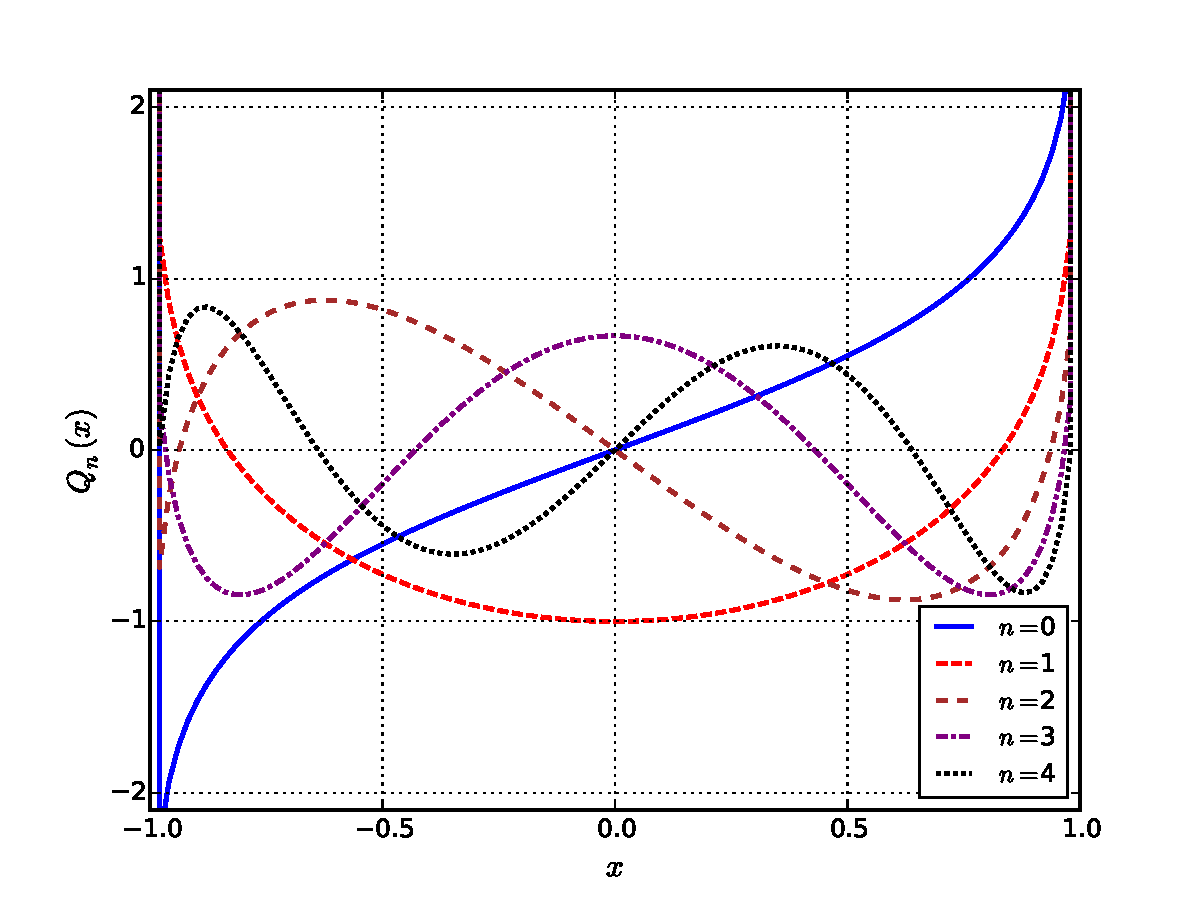
\includegraphics[angle=0,width=0.8\textwidth]{figs/fig-Legendre-Q.pdf}
\caption{Primeras cinco funciones de Legendre de segunda especie.}
\label{fig-Qn}
\end{figure}

\subsubsection{Propiedades de las funciones $Q_n(x)$}
\begin{itemize}
\item Paridad:
\begin{equation}
Q_n(-x)=(-1)^{n+1}Q_n(x)
\end{equation}

\item Valor en el origen:
\begin{equation}
Q_n(0)=
\begin{cases}
0, &  n\text{ par} \\
(-1)^{(n+1)/2}\frac{\left[\left(\frac{n-1}{2}\right)!\right]^2}{n!}2^{n-1}, & n\text{ impar}.
\end{cases}
\end{equation}

\item Valor en extremo del intervalo:
\begin{equation}
\lim_{x\to 1}Q_n(x)=+\infty .
\end{equation}
\end{itemize}



\section{Funciones asociadas de Legendre}

Podemos construir soluciones para la ecuaci'on \eqref{est22} a partir del siguiente teorema:
\begin{quote}
Si $P_Q^m(x)$ es una soluci'on de \eqref{est22} para un valor de $Q$ y $m$ datos, entonces 
\begin{equation}
u(x):=(1-x^2)^{(m+1)/2}\frac{d\ }{dx}\left[(1-x^2)^{-m/2}P_Q^m(x)\right]
\end{equation}
es tambi'en soluci'on de \eqref{est22}, pero con $m+1$ en lugar de $m$.
\end{quote}
Este resultado permite entonces generar nuevas soluciones, con distintos valores de $m$, a partir de una soluci'on conocida, y en particular a partir de $P_n^0$ que definimos como los polinomios de Legendre, $P_n^0(x):=P_n(x)$. A partir de esto, podemos definir las funciones asociadas de Legendre $P_n^m$ tales que
\begin{equation}\label{Pnm+1}
P_n^{m+1}(x)=(1-x^2)^{(m+1)/2}\frac{d\ }{dx}\left[(1-x^2)^{-m/2}P_n^m(x)\right]
\end{equation}
Iterando la relaci'on \eqref{Pnm+1} obtenemos, para $m=0,1,2,\cdots$, 
\begin{eqnarray}\label{Pnm}
P_n^m(x) =(1-x^2)^{m/2}\frac{d^m}{dx^m} P_n(x).
\end{eqnarray}
Por otro lado, las funciones con $m$ negativo pueden calcularse usando
\begin{eqnarray}
P_n^{-m}(x) = (-1)^m\frac{(n-m)!}{(n+m)!} P_n^m(x), \qquad m=0,1,2,\cdots.
\label{est29}
\end{eqnarray}

Ya que las funciones $P_n(x)$ son polinomios de orden $n$, vemos que existen soluciones $P_n^m(x)$ no nulas s'olo si
\begin{equation}
  m=0,\pm 1,\pm 2,\cdots,\pm n \qquad\Leftrightarrow\qquad
  |m|\leq n.
\end{equation}
Es decir, existen $2n+1$ valores permitidos de $m$ para cada $n=0,1,2,\cdots$.

\subsection{Expresiones expl'icitas}
\begin{align}
P_1^1(x) &= (1-x^2)^{1/2}, \\
P_2^1(x) &= 3x(1-x^2)^{1/2}, \\
P_2^2(x) &= 3(1-x^2), \\
P_3^1(x) &= \frac{3}{2}(1-x^2)^{1/2}(5x^2-1), \\
P_3^2(x) &= 15(1-x^2)x, \\
P_3^3(x) &= 15(1-x^2)^{3/2}. \\
\end{align}

\begin{figure}[H]
\centering
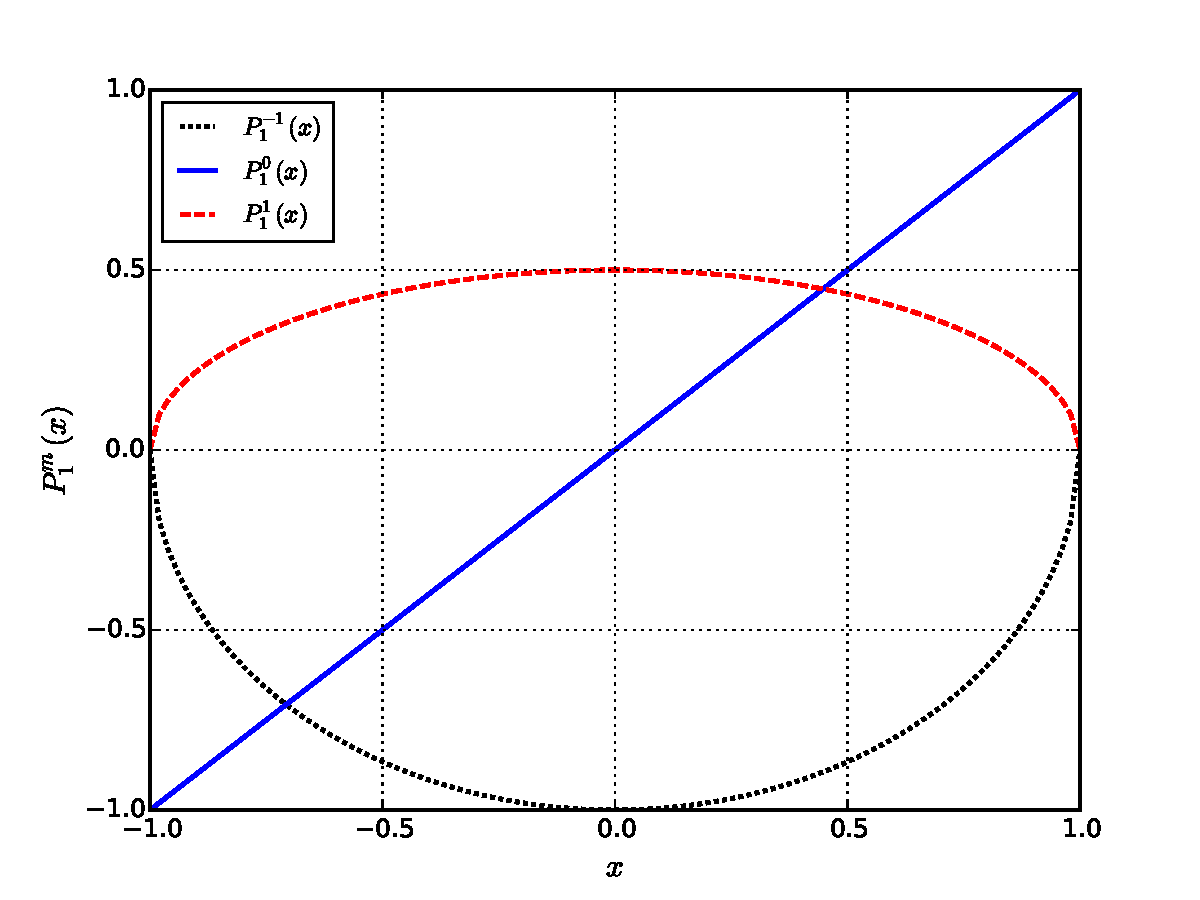
\includegraphics[angle=0,width=0.8\textwidth]{figs/fig-Legendre-Asoc-l-1.pdf}
\caption{Funciones Asociadas de Legendre: $n=1$.}
\label{fig-P1m}
\end{figure}
\begin{figure}[H]
\centering
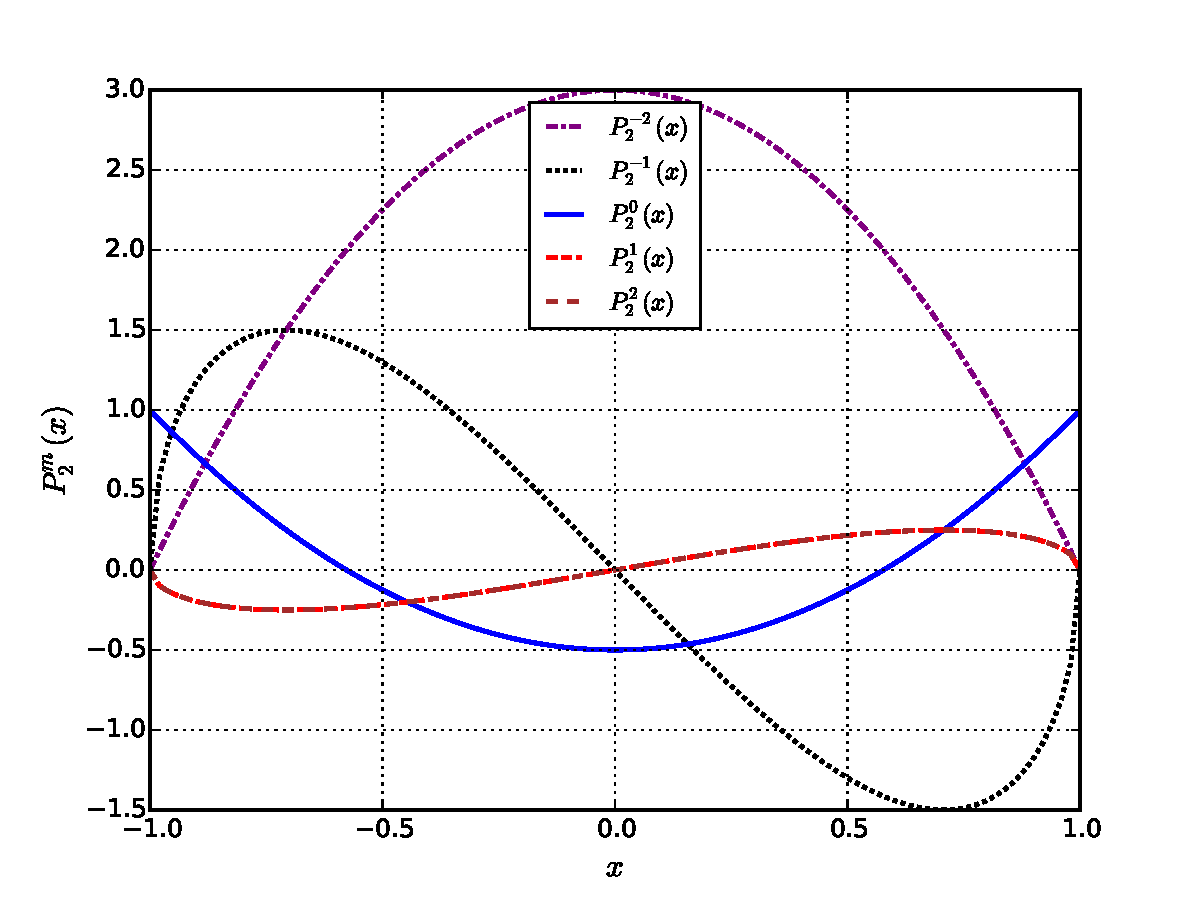
\includegraphics[angle=0,width=0.8\textwidth]{figs/fig-Legendre-Asoc-l-2.pdf}
\caption{Funciones Asociadas de Legendre: $n=2$.}
\label{fig-P2m}
\end{figure}
\begin{figure}[H]
\centering
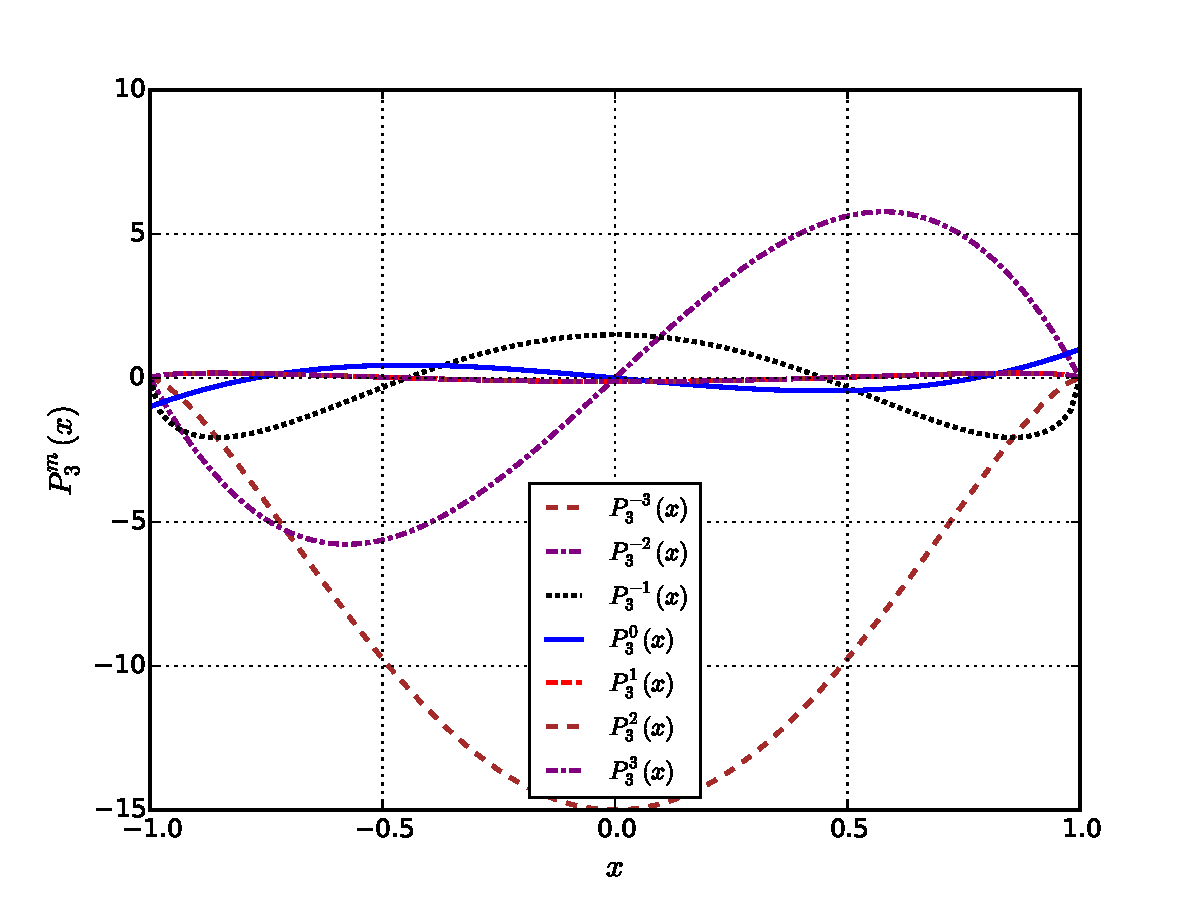
\includegraphics[angle=0,width=0.8\textwidth]{figs/fig-Legendre-Asoc-l-3.pdf}
\caption{Funciones Asociadas de Legendre: $n=3$.}
\label{fig-P3m}
\end{figure}
\subsection{F'ormula de Rodrigues}

\begin{equation}
P_{n}^{m}(x)=\frac{1}{2^{n}n!}(1-x^2)^{m/2}\frac{d^{m+n}}{dx^{m+n}}(x^2-1)^{n}.
\end{equation}

\subsection{Funci'on generadora}

\begin{equation}
\frac{(2m)! \, (1-x^2)^{m/2}}{2^{m}\, m! \, (1-2tx+t^2)^{m+1/2}} = \sum_{n=0}^{\infty} P_{n+m}^{m}(x) \, t^n
\end{equation}


\subsection{Relaciones de recurrencia}

\begin{equation}
(2n+1)xP_n^m=(n+m)P_{n-1}^m+(n+m+1)P_{n+1}^m
\end{equation}
\begin{align}
(2n+1)(1-x^2)^{1/2}P_n^m &= P_{n+1}^{m+1}-P_{n-1}^{m+1} \\
&= (n+m)(n+m-1)P_{n-1}^{m-1}-(n-m+1)(n-m+2)P_{n+1}^{m-1}
\end{align}

\subsection{Paridad}
A partir de \eqref{Pnm} y la paridad de los polinomios $P_n(x)$ encontramos que
\begin{equation}
P_n^m(-x)=(-1)^{m+m}P_n^m(x).
\end{equation}
Adem'as
\begin{equation}
P_n^m(\pm 1)=\left\{\begin{array}{cl}
(\pm 1)^n, & m=0\\
0, & m\neq 0
\end{array}\right..
\end{equation}
\subsection{Ortogonalidad}

\begin{equation}
\int_{-1}^{1}P_{n}^m(x)P_{n'}^m(x)\,dx=\frac{2}{2n+1}\frac{(n+m)!}{(n-m)!}\,\delta_{n,n'}.
\end{equation}



\section{Funciones Arm'onicas Esf'ericas}

 Volvemos ahora al problema original de encontrar las soluciones de la ecuaci'on
de Laplace. Usando (\ref{produkt1}), (\ref{Phim}) y el hecho que las funciones asociadas de Legendre son soluciones de \eqref{est22}, podemos expresar la soluci'on de \eqref{est20} como
 \begin{equation}
\Psi(r,\theta,\varphi)\propto R(r)P_l^m(\cos\theta)e^{im\varphi}.\label{est30}
 \end{equation}
Es por esto muy 'util y com'un definir las \textit{funciones arm'onicas
esf'ericas} $Y_l^m (\theta,\varphi)$ que, incorporando una normalizaci'on conveniente, son definidas por:
 \begin{eqnarray}
  Y_l^m (\theta,\varphi) := (-1)^m\sqrt\frac{2l+1}{4\pi}\cdot\sqrt\frac
   {(l-m)!}{(l+m)!}\cdot P_l^m(\cos\theta)\cdot e^{im\varphi}.\label{kugel1}
 \end{eqnarray}
  En la tabla \ref{tabelle1} se presentan los casos m'as usados.
\begin{table}[htbp]
\begin{tabular}{cc|c||cc|c}
  $l$ & $m$ & $Y_l^m $ & $l$ & $m$ & $Y_l^m $\\\hline
  0&0&$Y_0^0=\frac 1{\sqrt{4\pi}}$&2&2&$Y_2^2=\frac 14\sqrt\frac{15}{2\pi}
   \sen^2\theta e^{2i\varphi}$\\
  1&0&$Y_1^0=\sqrt\frac 3{4\pi}\cos\theta$&3&0&$Y_3^0=\sqrt\frac 7{4\pi}
  (\frac 52\cos^3\theta-\frac 32\cos\theta)$\\
  1&1&$Y_1^1=-\sqrt \frac 3{8\pi}\sen\theta e^{i\varphi}$&3&1&$Y_3^1=
  -\frac 14\sqrt\frac{21}{4\pi}\sen\theta(5\cos^2\theta-1)e^{i\varphi}$\\
  2&0&$Y_2^0=\sqrt\frac 5{4\pi}(\frac 32\cos^2\theta-\frac 12)$&3&2&$Y_3^2=
  \frac 12\sqrt\frac{105}{2\pi}\sen^2\theta\cos\theta e^{2i\varphi}$\\
  2&1&$Y_2^1=-\sqrt\frac{15}{8\pi}\sen\theta\cos\theta e^{i\varphi}$&3&3&$
  Y_3^3=-\frac 14\sqrt\frac{35}{4\pi}\sen^3\theta e^{3i\varphi}$
 \end{tabular}
\caption{Algunas funciones arm'onicas esf'ericas com'unmente usadas
($l,m=0,\ldots,3$).}
\label{tabelle1}
\end{table}

Como consecuencia de su definici'on, las funciones arm'onicas esf'ericas satisfacen las siguientes 'utiles
propiedades:
 \begin{itemize}
  \item \textit{Simetr'ia}:
   \begin{eqnarray}
    Y_l^{-m} = (-1)^m (Y_l^m)^*.\label{kugel2}
   \end{eqnarray}
  \item \textit{Ortonormalidad}:
  \begin{equation}
  \oint Y_l^m (\theta,\varphi)\cdot (Y_{l'}^{m'})^*(\theta,\varphi)\, d\Omega
=\int_0^{2\pi}\int_0^\pi Y_l^m (\theta,\varphi)  \cdot
(Y_{l'}^{m'})^*(\theta,\varphi)\, \sen\theta d\theta d\varphi   =
\delta_{ll'}\delta_{mm'},
\label{est33}
\end{equation}
 donde $d\Omega = \sen\theta d\theta d\varphi$ es el elemento de 'angulo
s'olido.

\item Como consecuencia de la ortogonalidad de las funciones $Y_l^m$, 'estas son linealmente independientes.

 \item Las funciones $Y_l^m $ forman un sistema completo de funciones. Toda
funci'on $f(\theta,\varphi)$ que satisface
\begin{equation}
    \int |f(\theta,\varphi)|^2 d\Omega <\infty,
\end{equation}
pueden ser desarrollada en t'erminos de funciones arm'onicas esf'ericas:
\begin{eqnarray}
f(\theta,\varphi) = \sum_{l=0}^\infty\sum_{m=-l}^l a_{lm}Y_l^m (\theta,\varphi),
\end{eqnarray}
con coeficientes $a_{lm}$ dados por
\begin{equation}
a_{lm}=\oint f(\theta,\varphi)(Y_{l}^{m})^*(\theta,\varphi)\,d\Omega.
\end{equation}

\item La completitud de $Y_l^m $ se expresa por:
\begin{equation}
    \sum_{l=0}^\infty\sum_{m=-l}^l (Y_l^m)^*(\theta,\varphi)
    Y_l^m (\theta',\varphi') = \delta(\varphi-\varphi')\delta(\cos\theta-
    \cos\theta').
\end{equation}
\item Las  funciones arm'onicas esf'ericas satisfacen
 \begin{eqnarray}
  \hat{L}^2(\theta,\varphi) Y_l^m  = l(l+1)Y_l^m ,
 \end{eqnarray}
donde $\hat{L}^2$ es el operador definido por
 \begin{eqnarray}
  -\hat{L}^2 :=
\frac{1}{\sen\theta}\frac{\partial}{\partial\theta}\left(\sen\theta\frac{
\partial}{\partial
  \theta}\right)+\frac 1{\sen^2\theta}\frac{\partial^2}{\partial \varphi^2}.
 \end{eqnarray}
 En otras palabras, las funciones $Y_l^m $ son funciones propias del operador
$\hat{L}^2$, con valor propio $l(l+1)$. En t'erminos de $\hat{L}^2$, podemos
escribir el operador de Laplace como:
 \begin{equation}
  \nabla^2 = \frac 1r\frac{\partial^2}{\partial r^2}\left( r \cdot\right) -
\frac{1}{r^2}\hat{L}^2.
\end{equation}
 \end{itemize}

\begin{figure}[H]
\centering
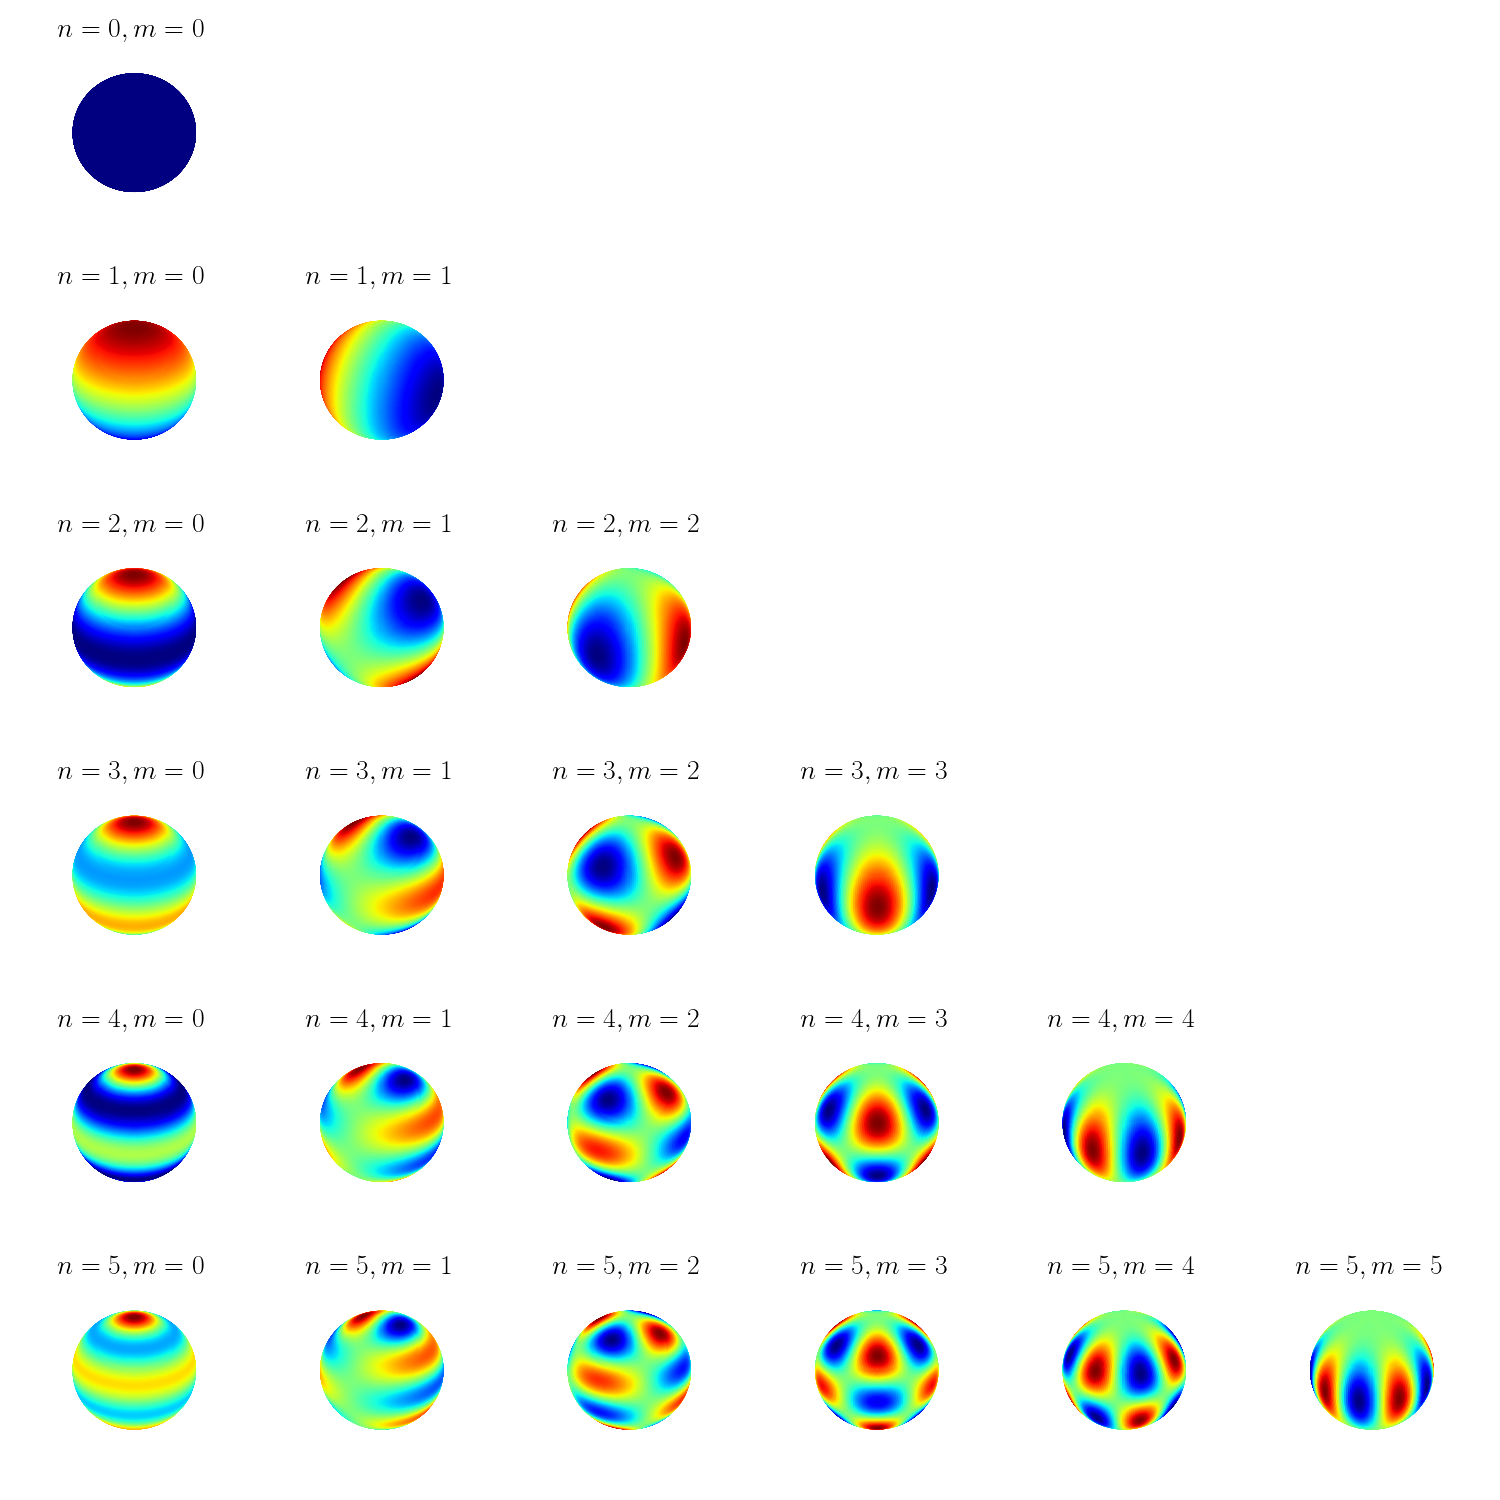
\includegraphics[angle=0,width=0.95\textwidth]{figs/fig-Aes3Dcolores.png}
\caption{Representaci'on gr'afica de (la parte real de) algunas funciones arm'onicas esf'ericas. C'odigo Python \href{https://github.com/gfrubi/FM2/blob/master/figuras-editables/Graficos-AE-esfera-colores.py}{aqu\'i}.}
\label{fig-Aes}
\end{figure}

\subsubsection{Teorema de adici'on de arm'onicos esf'ericos}
\begin{equation}
P_n(\cos\gamma) = \frac{4\pi}{2n+1} \sum_{m=-n}^n Y_n^m(\theta_1,\varphi_1)(Y_n^{m})^\ast(\theta_2,\varphi_2),
\end{equation}
donde $\gamma$ es el el 'angulo entre las direcciones definidas por los pares $(\theta_1,\varphi_1)$ y $(\theta_2,\varphi_2)$, por lo que est'an relacionados por
\begin{equation}
\cos\gamma = \cos\theta_1\cos\theta_2 + \sin\theta_1\sin\theta_2\cos(\varphi_1-\varphi_1).
\end{equation}

Un caso particular interesante de esta identidad se encuentra cuando ambas direcciones son iguales, de modo que  $\theta_1=\theta_2=\theta$ y $\varphi_1=\varphi_2=\varphi$, de modo que $\gamma=0$ y entonces
\begin{equation}
P_n(0) = \frac{4\pi}{2n+1} \sum_{m=-n}^n \left|Y_n^m(\theta,\varphi)\right|^2.
\end{equation}
De aqu'i obtenos directamente que
\begin{equation}
\sum_{m=-n}^n \left|Y_n^m(\theta,\varphi)\right|^2 = \frac{2n+1}{4\pi},
\end{equation}
lo que adem'as permite encontrar la siguiente cota superior para el m'odulo de las funciones arm'onicas esf'ericas:
\begin{equation}
\left|Y_n^m(\theta,\varphi)\right| \le \sqrt{\frac{2n+1}{4\pi}}.
\end{equation}

El teorema de adici'on es muy 'util en F'isica puesto que permite realizar expansiones de funciones como $\left|\vec{x}_1-\vec{x}_2\right|^{-1}$ que aparece com'unmente en distintas expresiones

Si $r_2<r_1$, con $r_1=\left|\vec{x}_1\right|$ y $r_2=\left|\vec{x}_2\right|$ entonces
\begin{equation}
\frac{1}{\left|\vec{x}_1-\vec{x}_2\right|} = \frac{1}{\sqrt{r_1^2+r_2^2-2r_1r_2\cos\gamma}} = \frac{1}{r_1}\frac{1}{\sqrt{1+t^2-2t\cos\gamma}},
\end{equation}
donde hemos definido $t:=r_2/r_1 <1$. Entonces
\begin{align}
\frac{1}{\left|\vec{x}_1-\vec{x}_2\right|} &= \frac{1}{r_1}\sum_{n=0}^\infty P_n(\cos\gamma)ṭ^n \\
&= \frac{1}{r_1}\sum_{n=0}^\infty t^n\frac{4\pi}{2n+1} \sum_{m=-n}^n Y_n^m(\theta,\varphi)(Y_n^{m})^\ast(\theta',\varphi')  \\
&= 4\pi \sum_{n,m}\frac{1}{2n+1}\frac{r_2^n}{r_1^{n+1}}Y_n^m(\theta,\varphi)(Y_n^{m})^\ast(\theta',\varphi').
\end{align}

\subsubsection{Ecuaci'on de Laplace y arm'onicos esf'ericos}
En el caso de la ecuaci'on de Laplace, podemos entonces usar el resultado en \eqref{loes2}, con $Q=n(n+1)$, para escribir una expresi'on general para la soluci'on (finita para $\theta=0$ y $\theta=\pi$), en coordenadas esf'ericas:
\begin{equation}
\Psi(r,\theta,\varphi)=\sum_{n,m}\left(A_{nm}r^n+\frac{B_{nm}}{r^{n+1}}\right)Y_n^m(\theta,\varphi).
\end{equation}